\section{Lossy Transmission Line}\label{lec:lec13}
In previous sections, we have discussed the lossless and low loss transmission line. We have studied the characteristics of lossless transmission line and have seen various applications of the lossless transmission line. In practice however, as frequency increases, the loss increases and the line becomes very lossy. In this section, we will see briefly the characteristics of a lossy line.

Obviously, if a line is very lossy then it is not a very efficient medium for transfer of power, so when we say a line is lossy in practice it is not very lossy but it is moderately lossy. Let us briefly examine the characteristic impedance and the propagation constant of a very lossy line, after which we will examine that of a moderately lossy line.

\subsection{Very Lossy Transmission Line}
For a very lossy line we will define the relationship between the primary constants as:
\begin{align*}
R\gg\omega L
\\G\gg\omega C
\end{align*}
For this line the characteristics impedance, $Z_0$ is given as
\begin{dmath}
Z_0 = \sqrt{\frac{R + j\omega L}{G + j\omega C}} \approx  \sqrt{\frac{R}{G}}
\label{eqn:xteristicsimplossy}
\end{dmath}
Equation~\eqref{eqn:xteristicsimplossy} is a real quantity. Similarly, the propagation constant given in equation~\eqref{eqn:propconstlossy} is also a real quantity.
\begin{align}
\gamma = \sqrt{(R + j\omega L)(G + j\omega C)} \approx \sqrt{RG}
\label{eqn:propconstlossy}
\end{align}
We observe that the characteristic impedance is real but the propagation constant is also real. Recall that when we studied the lossless transmission line the characteristic impedance was real, so looking at $Z_0$ does not tell you whether the line is very lossy or lossless. However, when we look at the propagation constant  $\gamma$ for a lossless line, $\gamma$ was purely imaginary ($\alpha$ = 0 and $\gamma$ = j$\beta$) but for  a very lossy line $\gamma$ is a real quantity($\beta$ = 0 and $\gamma$ = $\alpha$) which means there is no phase variation in space for whatever voltage or current variation we have on the transmission line. A lossy line does not represent the wave phenomena, so essentially the structure is not representing a medium which is carrying voltage or current waves. There is a voltage and current variation on the structure but it does not represent the wave phenomena instead you have a voltage that varies exponentially with the attenuation constant $\alpha$ = $\sqrt{RG}$ and there is no phase variation which implies no traveling wave.

Obviously, we are not interested in this case we are investigating. Let us however consider the case where $R$ and $G$ are comparable to $\omega L$ and $\omega C$ and we refer to this transmission line as the moderately lossy line.

\subsection{Moderately Lossy Transmission Line}Mathematically, the relationship between the primary constants can be expressed as follows:
\begin{align*}
R \approx \omega L\\
G \approx \omega C
\end{align*}
The propagation constant for the case of the moderately lossy line $\gamma$ is given in equation~\eqref{eqn:propconstmodloss} is a complex quantity.
\begin{align}
\gamma = \alpha +j\beta
\label{eqn:propconstmodloss}
\end{align}
Where $\alpha$ is comparable to $\beta$ since $R$ and $G$ are comparable to $\omega L$ and $\omega C$ respectively. From the voltage equation we derived in equation~\eqref{eqn:voltagefromload} written as follows:
\begin{dmath*}
V = V^+e^{\gamma l} + V^-e^{
-\gamma l}\quad\text{substituting }\gamma\text{ = }\alpha + j\beta
= V^+e^{\alpha l}e^{j\beta l} + V^-e^{-\alpha l}e^{-j\beta l}
\end{dmath*}
Such a traveling wave exponentially decays with the attenuation constant $\alpha$ and it has a phase constant $\beta$. Let us consider the forward traveling wave, $V^+e^{\alpha l}e^{j\beta l}$ we see that the wave exponentially grows towards the generator or in other words decays as we move towards the load.

Similarly, $V^-e^{-\alpha l}e^{-j\beta l}$ exponentially decays as we move towards the generator or exponentially grows towards the load. Depending upon the value of the ratio of $V^-$ and $V^+$ which is the reflection coefficient at the load point, $\Gamma_L$ the two traveling waves propagating in opposite directions decay or grow exponentially as we move towards the generator. We recall from the lossless case that the amplitude of $\Gamma_L$ was same at every point on the transmission line, however that is not true for the moderately lossy line because the amplitude of the reflected to incident wave varies with $\alpha l$, as $\Gamma$ is now a function of location on the transmission line.
\begin{figure}[h]
\centering
\includegraphics[width=1\linewidth]{"./graphics/moderately_lossy_TX_plot"}
\caption{A plot of the attenuation of the forward and backward traveling waves of the moderately lossy line from the load point.}
\end{figure}
\begin{figure}[h]
\centering
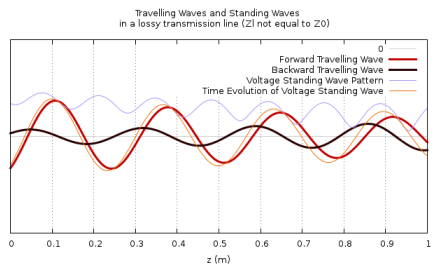
\includegraphics[width=1\linewidth]{./graphics/plot}
\caption{Standing wave of a moderately lossy line}
\end{figure}

The incident wave exponentially decays as we move towards the load and depending on the load value there is a certain reflection coefficient at the load so the value of the reflected wave exponentially decays as we we move towards the generator. So as we move to the generator the amplitude of the standing wave changes because at the load end the reflected wave dominates while at the generator end the incident wave dominates or the wave behaves more and more like a traveling wave instead of a standing wave.

From a different view it implies that if there is a large mismatch at the load side, as we move towards the generator the mismatch becomes weaker and the matching improves and we see an impedance at the generator end which is very close to the characteristic impedance $Z_0$ of the transmission line, because only the forward traveling wave is seen at the generator end. We conclude that for a lossy line, irrespective of what the load impedance is, there will always be a matching seen at the generator. But this is not a very good situation, because the power which is supplied by the generator is not delivered to the load. A substantial amount of power has been lost in the transmission line. So many times in transmission line design, a deliberately lossy line is introduced so that even in any experiment we connect some arbitrary load and get  some really strong reflections, at least these reflections will not go and damage the generator. So in this case the purpose certainly is not maximum power transfer but it is to protect the generator from any unwanted reflections.

\subsubsection{Using the Smith chart for lossy lines}
Let us examine the effect of a lossy line on the reflection coefficient of the transmission line. For the lossy line, the expression for the reflection coefficient is given as;
\begin{dmath*}
\Gamma{(l)} = \frac{V^-}{V^+}e^{-2\alpha l}e^{-j2\beta l}\quad\text{But, }\Gamma_L\text{ =}\frac{V^-}{V^+}
= \Gamma_Le^{-2\alpha l}e^{-j2\beta l}
\end{dmath*}
We would notice that if we know $\Gamma_L$, as we move towards the generator there will be a change \emph{but in what manner?} It is immediately clear when $\Gamma_L$ is expressed in this form $|\Gamma_L |e^{j\theta_L}$ where $\theta_L$ is the phase of the reflection coefficient at the load end and $|\Gamma_L|$ is the magnitude of the reflection coefficient at the load end.

Then,
\begin{dmath}
\Gamma{(l)} = |\Gamma_L|e^{-2\alpha l}e^{j(\theta_L-2\beta l)}
\label{eqn:gammalossy}
\end{dmath}
Equation~\eqref{eqn:gammalossy} shows that the total phase at a distance $l$ is $(\theta_L - 2\beta l)$ and the amplitude of the reflection coefficient at location $l$ is $|\Gamma_L|e^{-2\alpha l}$. As we move towards the generator $l$ is positive and the amplitude of the reflection coefficient goes on reducing exponentially.

The expression $|\Gamma_L|e^{j(\theta_L-2\beta l)}$ we have seen earlier in the complex gamma plane, traces a curve which is a circle. However, now there is the term $e^{-2\alpha l}$, the radius of the circle is reducing continuously and the expression $|\Gamma_L|e^{-2\alpha l}e^{j(\theta_L - 2\beta l)}$ essentially draws a spiral on the reflection coefficient plane as shown in figure~\ref{fig:lossygamma}(a).
\begin{figure}[h]
\centering
\includegraphics[width=1\linewidth]{"./graphics/lossy_gamma_temp"}
\caption{(a) A plot of the reflection coefficient on the $\Gamma$-plane. (b)Variation of the reflection coefficient along the transmission line towards the generator and the step value of $l = \frac{\lambda}{2}$ for $\Gamma(l)$ to approximate the spiral to a series of concentric circles.}
\label{fig:lossygamma}
\end{figure}

The VSWR which we have used to measure the contribution of the reflected wave, is not meaningful in the case of a moderately lossy transmission line because it is no more a characteristics of the load. It also has become a function of the transmission line characteristics, that is, the VSWR is a function of the length along the transmission line. Also, the standing wave expression is no longer a sinusoidal function and hence the separation between two adjacent minima is not exactly equal to $\frac{\lambda}{2}$. However, the separation is approximated to $\frac{\lambda}{2}$ because in practice most of the transmission lines have a loss which is reasonably small.

The process of analyzing moderately lossy line using Smith chart is hard without a software because the correct variations of the reflection coefficient or impedance variation need to be drawn. If the transmission line we are using has a small loss then we can approximate the spiral to a series of concentric circles. Each circle that follows is drawn after we move a distance of $\frac{\lambda}{2}$. From figure~\ref{fig:lossygamma}(b) we apply the approximation and a constant value of $\Gamma{(l)}$ is used for every $\frac{\lambda}{2}$ before correcting the magnitude of the reflection coefficient. The radii of the circles will differ by $\delta$ given by
\begin{dmath*}
\delta = \Delta \Gamma{(l)} = \Gamma_L(1 - e^{-2\alpha\cdot \frac{\lambda}{2}})
\end{dmath*}
A plot of these circles is shown in figure~\ref{fig:vswrlossy}, however, if we want to have a very accurate analysis then ideally we have to really draw this spiral on the Smith chart.
\begin{figure}[h]
\centering
\includegraphics[width=1\linewidth]{"./graphics/concentricVSWRcircles"}
\caption{Series of concentric circles of reflection coefficient $\Gamma{(l)}$ for $l = \frac{\lambda}{2},\lambda, \frac{3\lambda}{2}$ after we apply the approximation.}
\label{fig:vswrlossy}
\end{figure}

The analytic calculation of the impedance on a lossy line are as general as we have discussed earlier in the previous chapters. So those impedance transformation relationships using the hyperbolic cosines and sines are applicable for the calculation of the impedances on transmission line. Therefore, with this minor modification to the analysis, the Smith chart can be used for moderately lossy transmission lines.

\subsection{Characteristic Impedance and Propagation Constant measurement}
Here we would like to measure the characteristic impedance and the propagation constant which are the secondary constants. Normally for calculations of transmission lines, we generally do not estimate the primary constants rather we estimate the secondary constants. Assuming there is setup which can measure an unknown impedance at an unknown frequency. Then we can measure the characteristic impedance of a moderately lossy line or a low loss line. This measurement can be done by conducting a short circuit and open circuit test of a section of a transmission line. Consider a length of transmission line, $l$, one end of the transmission line is connected to the impedance measurement setup as shown in figure~\ref{fig:impmeasurement}.
\begin{figure}[h]
\centering
\includegraphics[width=1\linewidth]{"./graphics/impedance_measurement"}
\caption{Impedance measurement setup}
\label{fig:impmeasurement}
\end{figure}

We conduct the two test and measure the input impedances of this length of the transmission line by making the other end a short circuit and an open circuit. From the length we get $Z_{oc}$ and $Z_{sc}$. Recall,
\begin{align}
Z_{sc} = Z_0 \coth\gamma l\label{eqn:zsclossy}\\
Z_{oc} = Z_0 \tanh\gamma l\label{eqn:zoclossy}
\end{align}
So with $l$ known we can measure these impedances. We can get the expression for the characteristic impedance and the propagation constant as folows;

Multiplying equation~\eqref{eqn:zsclossy} and~\eqref{eqn:zoclossy}, gives
\begin{dmath*}
Z_{sc}Z_{oc}
= Z_0\tanh\gamma l Z_0\coth\gamma l
= {Z_0}^2\quad\text{Recall, }\coth\theta\text{ = }\frac{1}{\tanh\theta}
\end{dmath*}
Therefore,
\begin{equation}
Z_0 = \sqrt{Z_{oc}\cdot Z_{sc}}
\label{eqn:xteristicsimplossy2}
\end{equation}
Also dividing equation~\eqref{eqn:zsclossy} by~\eqref{eqn:zoclossy} gives
\begin{dmath*}
\frac{Z_{sc}}{Z_{oc}} = \frac{\tanh\gamma l}{\coth\gamma l} 
= \tanh^2\gamma l
\end{dmath*}
Thus,
\begin{dmath*}
\tanh\gamma l = \sqrt{\frac{Z_{sc}}{Z_{oc}}}\quad\text{Let }\sqrt{\frac{Z_{sc}}{Z_{oc}}}\text{ = }A
= A\quad\text{But }\tanh \theta\text{ = }\frac{e^\theta - e^{-\theta}}{e^\theta + e^{-\theta}}
=\frac{e^{\gamma l} - e^{-\gamma l}}{e^{\gamma l} + e^{-\gamma l}}
\end{dmath*}
Dividing the numerator and denominator by $e^{-\gamma l}$
\begin{dmath*}
\tanh\gamma l = \frac{(e^{\gamma l} - e^{-\gamma l})/e^{-\gamma l}}{(e^{\gamma l} + e^{-\gamma l})/e{-\gamma l}}
= \frac{e^{2\gamma l} - 1}{e^{2\gamma l} + 1} = A
\end{dmath*}
Making $e^{2\gamma l}$ the subject of the formula
\begin{align*}
e^{2\gamma l} &= \frac{1 +A}{1 - A}\equiv \Re e^{j\theta}\\
e^{2(\alpha + j\beta)l} &\equiv \Re e^{j\theta}\quad\text{Since }\gamma = \alpha + j\beta
\end{align*}
\begin{align}
e^{2\alpha l}e^{j2\beta l} \equiv \Re e^{j\theta}
\label{eqn:generaleqnimp}
\end{align}
\begin{align*}
\Re = \left|\frac{1 + A}{1 - A}\right|\\ \Rightarrow e^{2\alpha l} = \left|\frac{1 + A}{1 - A}\right|
\end{align*}
\begin{align}
\alpha = \frac{1}{2l}\ln\left|\frac{1 + A}{1 - A}\right|
\end{align}
Hence attenuation constant can be calculated once $A$ is known, where $A = \sqrt{\frac{Z_{sc}}{Z_{oc}}}$. Next we find $\beta$ from equation~\eqref{eqn:generaleqnimp}.
\begin{align*}
e^{j2\beta l} = e^{j\theta}
\end{align*}
However, now there is an ambiguity of multiples of $2\pi$ since the same magnitude of a complex variable can be gotten after we transverse $2\pi$ in either direction. So, $e^{2\beta l} = e^{(\theta \pm 2m\pi)}$ and
\begin{align}
\beta = \frac{1}{2l} (\theta \pm 2m\pi)
\end{align}
Where $m$ is an integer quantity and $\theta$ is the angle of $\frac{1 + A}{1 - A}$. Hence $\beta$ is calculated with some level of uncertainty in terms of what should be $m$ for our solution. The calculation of attenuation constant as we have noticed is straight forward from the short circuit and open circuit test.

If we take a length of line to be $\frac{\lambda}{2}$, it is clear that $m = 0$ for sure, and then we have a unique value of $\beta$ or a correct value for $\beta$. However if we take $l < \frac{\lambda}{2}$, especially at high frequencies, the length of the line is very small and since attenuation is very small on transmission line the $\alpha$ generally is very small. So for a small length of transmission line, the losses are not very significant, as a result when you try to calculate the equivalent value of $\alpha$, you do not get a very accurate value for $\alpha$, because of the small length of transmission line which is less than $\frac{\lambda}{2}$. The line behaves more or less like a lossless line. Hence the equation of attenuation constant becomes rather unreliable if we take a small length of line which is less than $\frac{\lambda}{2}$.

On the other hand to improve the reliability of $\alpha$, if we take a long length of cable, suddenly we have many periods of the wavelength on this transmission line. While $\alpha = \frac{1}{2l}\ln\left|\frac{1 + A}{1 - A}\right|$ becomes more accurate at this point, we have to resolve the $\beta = \frac{1}{2l} (\theta \pm 2m\pi)$ problem of many solutions within the line length in the measurement of the phase constant.

To resolve this issue, using the setup we take measurement at two frequencies. The first measurement of $Z_{oc}$ and $Z_{sc}$ is taken at one frequency  to get $\beta$ which is ambiguous with $2m\pi$. Then the frequency is changed slowly so that we get same value of phase variation. At  that point the number of cycles which we have on the transmission line has just changed by one. So by slowly changing the frequency and making sure only one cycle change takes place in $\theta$, then the $m$ is changed from $m$ to $m + 1$ and then we get a value of $\beta$. From here the two values of $\beta$ is used to find the correct value of $\beta$ as  follows:

Let $f_1$ and $f_2$ be the frequencies in which we carried out the measurement of  $Z_{oc}$ and $Z_{sc}$, let us assume at $f_1$ we get  $Z_{oc}$ and $Z_{sc}$ and get
\begin{equation}
\beta_1= \frac{1}{2l}(\theta + 2m\pi)\footnote{Taking the positive increments of $\theta$}
\label{eqn:betaf1}
\end{equation}
Next we slowly change frequency to get to where $Z_{oc}$ and $Z_{sc}$ again become same. Assuming that the length of the transmission line is very large, by changing the frequency by a small amount, the attenuation constant does not change significantly. What it essentially means is that if we increase the frequency by a small amount, the number of wavelengths set up on the line are changed by a cycle$(\frac{\lambda}{2})$, then the loss does not change significantly and that is the reason we get the same value of $Z_{oc}$ and $Z_{sc}$.

At $f_2$,
\begin{equation}
\beta_2 = \frac{1}{2l}(\theta + 2(m + 1)\pi)
\label{eqn:betaf2}
\end{equation}
Subtracting equation~\eqref{eqn:betaf1} from~\eqref{eqn:betaf2}
\begin{dmath*}
\beta_2 - \beta_1 = \frac{(m + 1)\pi}{l} - \frac{m\pi}{l}
= \frac{\pi}{l}
\end{dmath*}
$\beta_2$ and $\beta_1$ are related to the velocity or wavelength of the transmission line as $( \beta = \frac{2\pi}{\lambda} = \frac{2\pi}{\frac{v}{f}} = \frac{2\pi f}{v})$ so that
\begin{align*}
\frac{2\pi f_2}{v} - \frac{2\pi f_1}{v} = \frac{\pi}{l}\\
\frac{2\pi(f_2 - f_1)}{v} = \frac{\pi}{l}\\
\beta = \frac{2\pi f}{v} = \frac{2\pi f}{2l(f_2 - f_1)}
\end{align*}
\begin{align}
v = 2l(f_2-f_1)
\label{eqn:velocitylossy}
\end{align}
But $\beta = \frac{2\pi f}{v}$, so substituting equation~\eqref{eqn:velocitylossy} gives:
\begin{align*}
\beta = \frac{2\pi f}{2l(f_2 - f_1)}
\end{align*}
\begin{align}
\beta = \frac{\pi f}{l(f_2 - f_1)}
\end{align}
So what we have done is to carry out this measurement at two frequencies which are closely spaced in such a way that changing the frequency from $f_1$ to $f_2$, the number of cycles on the section of the line is only increased by one. Then from there we calculate the value of the velocity of the wave in the transmission line and then we get the phase constant.

At this point one may ask \emph{why are we estimating the velocity on the line? Does the wave not travel with the velocity of light on the line or if we know $\beta$ can we not find what $\lambda$ is and then find the velocity?} In fact the problem is exactly opposite. The problem depends on the structure of the line, the velocity of the wave actually changes, FREQUENCY is the one that is SACRED but depending upon propagation characteristics, velocity changes or the wavelength changes and therefore the phase constant changes. So it is not that we know the wavelength from the velocity and we are trying to find out $\beta$. In fact $\beta$ is the quantity which is the most unknown quantity. So for a given structure we first estimate the value of $\beta$, then wavelength ($\frac{2\pi}{\beta}= \lambda$) and velocity ($\lambda f = v$). So in practice, the measurement of the attenuation constant and the phase constant have to go through all these steps that have been stated.

This is the method which we mentioned in the open or short circuit test. This is the most widely used test in practice for measuring the characteristic impedance and propagation constant of the line. Of course there are certain practical difficulties, when we try to apply the open circuit or short circuit to the end of the transmission line, even if you short the two conductors of a transmission line, there will always be some conductance at the end. If the two ends are left open for the open circuit test, there will be some fringing capacitance at the end of the line. So realizing a perfect open or short circuit at very high frequency, is not that straight forward. People make extra effort to develop modules called short circuit modules and open circuit modules which can be connected to the end of the line to realize a good open or short circuit.
\begin{figure}[h]
\centering
\includegraphics[width=1\linewidth]{"./graphics/Short circuit load"}
\caption{Open circuit and short circuit load}
\end{figure}

In this chapter, we have discussed the characteristics of a lossy line and that of a moderately lossy line. We have also studied how to make use of Smith chart for this moderately lossy transmission line and the use of a practical method that brought in $\delta$ change for $\frac{\lambda}{2}$ movement in length when drawing the approximation for the reflection coefficient on the gamma plane. Lastly, we saw a practical method for estimating the characteristics impedance and complex propagation constant of a transmission line.

\section*{Exercises}
\begin{ExerciseList}
\Exercise[label={ex131}]
A lossy transmission line has a characteristic impedance of $50\varOmega$ and a propagation constant of $0.02 + j0.1$. Find the wavelength, velocity of propagation and the loss in dB/m.
\Answer[ref={ex131}]
% \begin{align*}
% \alpha &= 0.02 m^{-1}\\
% \beta &= 0.1 m^{-1}\\
% Z_0 &= 50\varOmega\\
% \gamma &= \alpha + j\beta\\
% \lambda &= \frac{2\pi}{\beta} = \frac{2\pi}{0.1} = 20\pi m\\
% v &= \lambda f = 20\pi f\\
% \text{Loss} &= 20\log_{10}e^{-2\alpha l} = 20\log_{10}e^{-2\times 0.02\times l} = 20\log_{10}e^{-0.04l}\\
% &= -0.086l dB/m
% \end{align*}
(a) The wavelength is $20\pi$m, (b) the velocity of propagation is $20\pi f$ and (c) the loss is $-0.086l$dB/m.
\end{ExerciseList}